
\section{\biochem}
\label{sec:juliaball}
In this work, we sought to redesign the popular \ball package for molecular analysis and simulation. This section initially examines reasons for a redesign in Julia, followed by a description of the core implementation of \biochem closing with the benchmark results. 

\subsection{Reasons for a redesign or \textit{why Julia?}}

While the design goals and the need for an open-source framework with the rich functionality such as \ball's  is still present, the realization of the main design principles of \ball are highly dependent on the choice of the programming language. From today's perspective in particular with regard to its purpose as a platform for rapid application development~(RAD), the usage of C++ may be considered sub optimal. \\
As for many scientific software packages, the development times for applications play a crucial role for the acceptance and usability of the underlying software. For example, a great deal of time may have to be spend by installing the library with its dependencies. Although the CMake build system has been integrated in version 1.3, setting up the library is a highly non-trivial task. Additionally, the development times are massively influenced by the knowledge of the used programming language. As a low-level language, C++ is known to require more time to be learned compared to scripting languages such as Python \cite{Ousterhout1998}. 
Even with the additional Python bindings, the integration of new functionality is still not straightforward. In contrast, the implementation of new features is typically associated with the addition of massive amounts of boilerplate code. This applies to an even greater extent, in cases where portability to different platforms and compiler settings have to be supported. \\
Consequently, \ball itself can be considered as a textbook example for the two language problem, which is very common for scientific computing project. In the latter, the core functionality is often implemented in a low-level programming language, ensuring the required performance, while higher-level programming languages are used for user-friendly interfaces to the core functionalities. Julia is exactly developed for these situations and guarantees the numerical stability and accuracy required for molecular mechanics applications \cite{Julia_what, Julia_accomplish}.\\ 
Nevertheless, it is important to keep in mind, that back in 1996 and still in 2010, C++ was the best choice for the implementation of \ball. \\
Switching our development from C++ to Julia has greatly simplified conforming the design goals denoted in Table~\ref{table1_design_goals}: 
\begin{itemize}
	\item Ease of use: \biochem's source code provides a better readability  as the usage of Julia does not produce so much boilerplate code compared to \ball. The integration of documentation, basic tutorials and test cases facilitates the introduction to \biochem, not to mention the trivial installation via Julia's Package manager. 
	
	\item Openness: Just like the installation, the integration of external tools to \biochem is straightforward. Our well documented framework allows the integration of own applications seamlessly. 
	
	\item Robustness: One of the strength of Julia is the integrated unit testing functionality allowing to test implemented code on the fly. \biochem has been carefully developed with accompanying test case for the core structures as well as for the functionalities ensuring non-faulty behavior using \texttt{TestItemRunner.jl}\cite{TestItemRunner}. Benchmark test cases are implemented in order to assess performance of typical tasks with the help of \texttt{BenchmarkTools.jl} and \texttt{Pkgbenchmark.jl} \cite{BenchmarkTools.jl-2016, PkgBenchmark}. The results of the benchmark study are described in section below. 
	
	\item Functionality: \biochem implements a set of standard data structures for molecular entities and already provides different functionalities based on these including import of structures stored in PDB, pubchem or hin files, molecular mechanics more precisely an interface for force fields and an Amber implementation, structure minimization algorithms. The interfaces are designed in a way that facilitates adoption e.g., implementation of own force field or changing an optimizer for the structure minimization. 
\end{itemize}

\subsection{The core representation}
In addition to the four original design goals, we sought to make \biochem comparable in performance to \ball. When working with structural data of molecular entities such as proteins, or nucleic acid molecules (DNA/RNA), the representation of atoms play an important role. \\
More precisely, we decided to put the \texttt{System} at the center of every application in \biochem. If the system is not defined explicitly, it will be generated by default. As shown in Figure~\ref{fig:biochem_uml}, the system contains data structures for the representation of atoms, bonds, molecules, chains, residues, nucleotides and fragments as soon as they are generated explicitly (see code listing ~\ref{lst:code-water})  or populated by reading files (see code listing ~\ref{lst:rmsd-and-amber}).   \\

The representation of an atom with their position, velocity and force contributes substantially to the efficiency of the entire framework. Therefore, careful attention has been given to the implementation of the underlying data structure. Due to its popularity and intuitive usage, a preliminary attempt consisted of a representation using \texttt{DataFrames.jl} \cite{Bouchet-Valat2023}. However, we decided to move to a costume implementation of the \texttt{Tables.jl} interface \cite{BouchetValat2018}. The costume implementation enabled more flexibility regarding the design of the interface and in addition, initial benchmarks indicated a better performance (data not shown). \\
\todo{Why is more flexibility needed?}
\todo{Tables interface allows to be converted to BioStructures.jl stuff and so on}
The Table~\ref{table2_benchmark} lists the results of a benchmark study comparing the time needed for typical core functionalities in \ball and \biochem. It is evident \biochem is on par with its C++ predecessor.
\begin{figure*}[t]
	\centerline{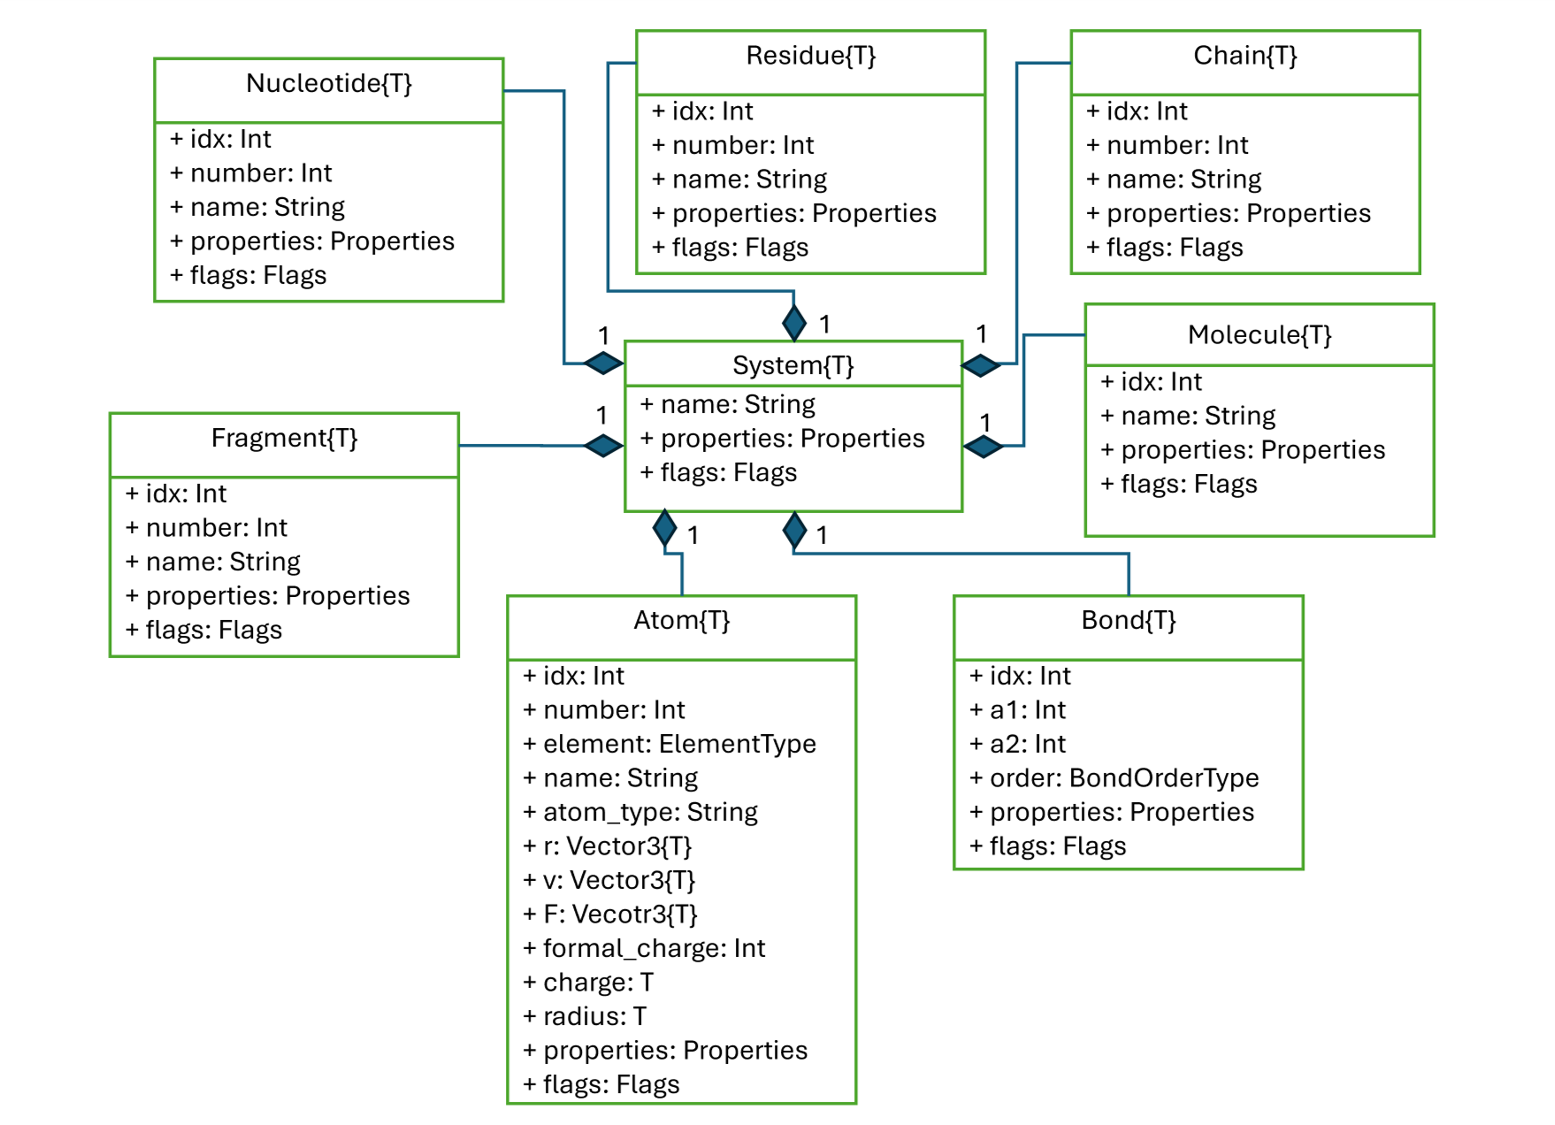
\includegraphics[width=15cm]{gfx/uml.png}}
	\caption{UML-Diagramm of the core of \biochem . In the center resides the \texttt{System} interface. All other functionalities are grouped around that core piece. Only the most important functionalities of each class are  shown.}
	\label{fig:biochem_uml}
\end{figure*}

\begin{table}
	\tbl{Example tasks and the required time}{
		\begin{tabular}{|l|c|c|}\hline
			Description & \ball & \biochem \\
			tba & tba & tba\\hline
			tba & tba & tba \\\hline
		tba	& tbal & tba \\ \hline
	\end{tabular}}
\label{table2_benchmark}
\end{table}